%Chapter 2
\chapter{Literature Review}\label{sec:literature_review}

This chapter examines the theoretical foundations underlying the empirical analysis presented in this thesis, with particular attention to a fundamental tension that shapes modern startup strategy. The literature review is organized around three core domains: technical debt conceptualization and measurement, development velocity assessment in software engineering, and venture capital success metrics. However, these domains present conflicting strategic imperatives. Traditional software engineering principles advocate for rigorous technical debt management as essential for long-term sustainability, while the venture capital ecosystem—particularly during the zero interest-rate policy era—has explicitly rewarded rapid execution and market capture, often at the expense of code quality. A critical synthesis of recent and foundational literature from these fields establishes the conceptual framework necessary to investigate whether technical debt represents a strategic liability or a competitive tool in venture-backed software companies.

\section{Defining and Measuring Technical Debt: The Traditional Engineering Perspective}\label{sec:technical_debt_literature}

The discourse surrounding technical debt provides the foundation for understanding the engineering perspective on quality versus speed trade-offs. This section examines the evolution of the technical debt metaphor, its various manifestations, and the prevailing methodologies for its measurement, while positioning these concepts within the traditional software engineering paradigm that views debt as fundamentally problematic.

\subsection{The Debt Metaphor and Its Evolution}
The concept of technical debt, first articulated by Ward Cunningham in 1992, has evolved from a simple metaphor for explaining design shortcuts to a comprehensive framework for understanding the long-term implications of software development decisions \citep{cunningham1992wycash}. Cunningham's original formulation emphasized that shipping code that is not ``quite right'' is analogous to taking on financial debt. This initial act of ``borrowing'' against a clean, optimal design allows for immediate product delivery but incurs ``interest payments'' in the form of increased development effort and complexity in all future work until the ``principal'' is repaid through refactoring. The metaphor's power lies in its ability to frame a technical issue in clear business terms, suggesting that not all debt is inherently negative; it can be a strategic tool for leveraging market opportunities \citep{seaman2012using}. This strategic dimension becomes critical when startups face time-sensitive competitive windows. In fast-moving markets, the opportunity cost of delayed market entry can far exceed the interest payments on technical debt \citep{curtis2012estimating}. The debt metaphor thus captures a fundamental startup trade-off: accepting future maintenance costs (interest) to accelerate feature delivery and secure market position today. This calculus intensifies in venture-backed software companies, where securing subsequent funding rounds often depends on demonstrating rapid user growth and market traction within narrow windows \citep{lee2024startups}. The metaphor therefore extends beyond software engineering to encompass the broader strategic question of resource allocation under conditions of capital scarcity and competitive pressure.

Martin Fowler's influential ``Technical Debt Quadrant'' provides a more nuanced taxonomy, distinguishing between different types of technical debt based on whether it is deliberate or inadvertent, and prudent or reckless \citep{fowler2009technical}. Deliberate and prudent debt represents a conscious, strategic decision to prioritize speed over perfection to meet a critical deadline, with a full understanding of the future costs. This contrasts with reckless and inadvertent debt, which arises from poor practices or lack of awareness and offers no strategic upside. Importantly, even within this framework, the traditional engineering perspective maintains that debt should be temporary and strategically managed—a view that, as we will explore, may be challenged by the unique pressures of venture-backed startups during periods of abundant capital.

\begin{figure}[htbp]
\centering
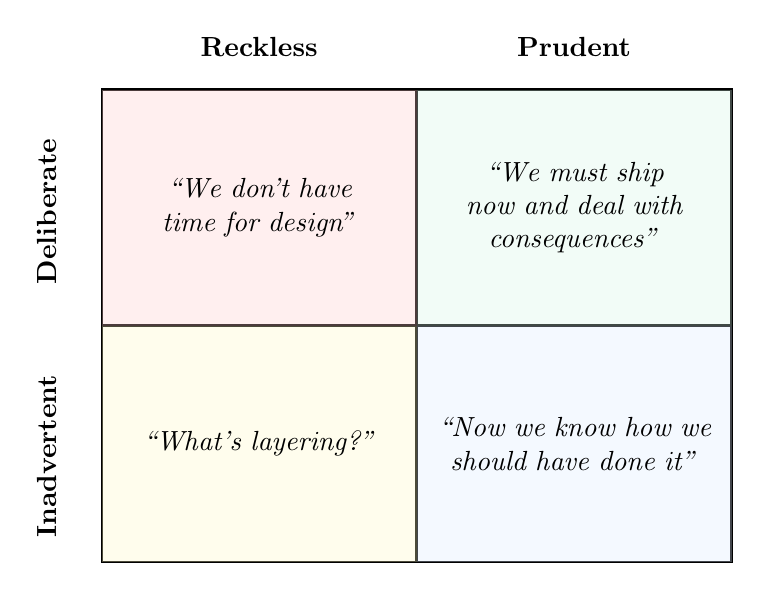
\begin{tikzpicture}[scale=1]
    % Define colors
    \definecolor{lightblue}{RGB}{219, 234, 254}
    \definecolor{lightgreen}{RGB}{213, 244, 230}
    \definecolor{lightyellow}{RGB}{254, 249, 195}
    \definecolor{lightred}{RGB}{254, 202, 202}
    
    % Draw the main axes
    \draw[very thick] (-4,0) -- (4,0);
    \draw[very thick] (0,-3) -- (0,3);
    
    % Draw quadrant boxes
    \draw[thick] (-4,-3) rectangle (0,0);  % Bottom-left
    \draw[thick] (0,-3) rectangle (4,0);   % Bottom-right
    \draw[thick] (-4,0) rectangle (0,3);   % Top-left
    \draw[thick] (0,0) rectangle (4,3);    % Top-right
    
    % Fill quadrants with colors
    \fill[lightred, opacity=0.3] (-4,0) rectangle (0,3);      % Top-left: Reckless & Deliberate
    \fill[lightgreen, opacity=0.3] (0,0) rectangle (4,3);    % Top-right: Prudent & Deliberate
    \fill[lightyellow, opacity=0.3] (-4,-3) rectangle (0,0); % Bottom-left: Reckless & Inadvertent
    \fill[lightblue, opacity=0.3] (0,-3) rectangle (4,0);    % Bottom-right: Prudent & Inadvertent
    
    % Simple axis labels
    \node[above] at (-2,3.3) {\textbf{Reckless}};
    \node[above] at (2,3.3) {\textbf{Prudent}};
    \node[left, rotate=90] at (-4.7,2.5) {\textbf{Deliberate}};
    \node[left, rotate=90] at (-4.7,-0.5) {\textbf{Inadvertent}};
    
    % Quadrant content - Top-left (Reckless & Deliberate)
    \node[text width=3.5cm, align=center] at (-2,1.5) {
        \textit{``We don't have time for design''}
    };
    
    % Quadrant content - Top-right (Prudent & Deliberate)
    \node[text width=3.5cm, align=center] at (2,1.5) {
        \textit{``We must ship now and deal with consequences''}
    };
    
    % Quadrant content - Bottom-left (Reckless & Inadvertent)
    \node[text width=3.5cm, align=center] at (-2,-1.5) {
        \textit{``What's layering?''}
    };
    
    % Quadrant content - Bottom-right (Prudent & Inadvertent)
    \node[text width=3.5cm, align=center] at (2,-1.5) {
        \textit{``Now we know how we should have done it''}
    };
    
\end{tikzpicture}
\caption{Fowler's Technical Debt Quadrant}
\label{fig:fowler_quadrant}
\end{figure}

\subsection{Types and Manifestations of Technical Debt}

Technical debt is not a monolithic concept; it manifests in numerous forms throughout the software development lifecycle. While code debt is the most commonly measured, other forms can have equally significant impacts on a startup's trajectory. A synthesized taxonomy based on recent literature includes \citep{morgenthaler2012searching}:

\textbf{Code Debt} encompasses violations of coding standards, high cyclomatic complexity, duplicated code, and other ``code smells'' that degrade readability and maintainability \citep{arcelli2012investigating}. This represents the most immediately visible form of technical debt, readily detected through automated analysis tools.

\textbf{Architectural Debt} involves suboptimal design decisions at the system level that constrain future scalability and modification. This form of debt is often the most costly to repay, as it may require fundamental restructuring of system components.

\textbf{Test Debt} manifests as inadequate or missing test suites, leading to increased risk of bugs and higher cost of validation for new features. In startup environments, test debt is frequently accumulated due to time pressures for rapid deployment.

\textbf{Infrastructure and Build Debt} includes non-automated deployment processes, inconsistent development environments, and brittle build systems, all of which introduce friction into the development cycle and slow down velocity \citep{morgenthaler2012searching}.

The primary causes of technical debt align closely with pressures inherent in startup environments. Time pressure to meet market windows or investor milestones represents the most cited cause \citep{li2015systematic}. This is compounded by business pressure for new features, volatility in requirements, and resource constraints that limit the availability of skilled personnel or time for proper refactoring. These causes highlight the fundamental tension: the very conditions that define startup success—rapid iteration, resource constraints, and urgent market pressures—are precisely those that the traditional engineering perspective identifies as debt-inducing.

\subsection{Measurement Approaches and Strategic Context}

The automated measurement of technical debt relies fundamentally on static code analysis—the examination of source code without executing it. This approach provides the scalability necessary for large-scale empirical research while offering objective, repeatable measurements of code quality. However, the relationship between static analysis outputs and actual strategic impact in venture-backed environments requires careful consideration, as the strategic calculus during the \ac{ZIRP} era fundamentally altered traditional quality-cost trade-offs.

\subsubsection{Static Analysis Foundations}

The theoretical justification for using static analysis as a proxy for technical debt stems directly from Cunningham's original debt metaphor \citep{cunningham1992wycash}. Static analysis tools systematically identify patterns in source code that correlate with poor maintainability, increased complexity, and higher likelihood of defects—precisely the characteristics that Cunningham described as incurring ``interest payments'' on technical debt.

However, static analysis primarily captures surface-level quality indicators that may not reflect the strategic debt accumulation patterns most relevant to startup velocity and funding outcomes. Architectural debt, arising from suboptimal system-level design decisions, often represents the most costly form of technical debt to remediate \citep{martini2014architecture}, yet remains largely invisible to conventional static analysis tools.

\subsubsection{Economic Modeling and Strategic Context}

The economic framing of technical debt becomes particularly relevant in venture-backed environments, where engineering decisions are explicitly evaluated against financial constraints and investor expectations. The ability to quantify technical debt in monetary terms—time costs, development effort, delayed features—enables direct comparison with the capital abundance and growth pressures that define startup strategic contexts.

During the \ac{ZIRP} era, abundant capital fundamentally altered the strategic calculus surrounding quality trade-offs. Traditional software engineering assumes that technical debt's ``interest payments'' represent unavoidable future costs that rational actors should minimize. However, when external funding can continuously subsidize these interest payments, and when the penalty for slow market execution exceeds the long-term costs of debt accumulation, the strategic optimal may involve accepting higher debt levels in exchange for accelerated development velocity.

\subsubsection{Strategic Implications for Venture-Backed Development}

This measurement constraint has profound implications for understanding technical debt's strategic role in venture execution. Startups classified as ``high debt'' based on static analysis may actually maintain clean architecture and robust testing practices—the forms of technical health most crucial for sustaining rapid development velocity. Conversely, companies with excellent code-level metrics may harbor architectural decisions that fundamentally constrain their ability to scale, particularly relevant given the ``blitzscaling'' imperative during the \ac{ZIRP} era.

The challenge extends beyond tool limitations to fundamental questions about what constitutes ``strategic debt'' in venture-backed environments. Traditional software engineering frameworks assume that all forms of technical debt eventually impose velocity constraints, but this assumption may not hold when external capital can continuously subsidize the costs of code-level inefficiencies while market timing pressures make architectural perfection a secondary concern.

Nevertheless, code-level debt represents the most objectively measurable and comparable form of technical debt across organizations, providing a standardized foundation for empirical analysis. The specific implementation details and validation approaches for measuring technical debt in this research context are detailed in \autoref{sec:analysis_pipeline}, where the automated analysis pipeline and tool selection criteria are comprehensively addressed.

\section{Development Velocity \& Agility in Software Engineering}\label{sec:velocity_literature}

Development velocity became a central concept with the rise of agile methodologies, which prioritize delivery speed and iterative development over the rigid, plan-driven approaches of traditional software engineering \citep{beck2001agile}. However, the measurement and interpretation of velocity takes on fundamentally different meanings when considered through the lens of venture capital evaluation criteria, as will be explored in the following section.

\subsection{Conceptualizing and Measuring Velocity}

Within agile frameworks like Scrum, velocity is traditionally the number of ``story points'' a team completes per sprint \citep{sutherland2004agile}. While useful for a single team's internal planning, story points are subjective and not comparable across different organizations, limiting their utility for external research \citep{cohn2005agile}. Consequently, researchers have turned to objective, repository-derived data to create standardized velocity metrics. This approach, exemplified by the Cloud Native Computing Foundation's (CNCF) ``project velocity'' metric, synthesizes multiple activity indicators to provide a holistic view of project momentum \citep{cncf2022velocity}. Recent work by Lee \& Kim (2024) confirms that such objective measures, derived from job postings and development activity, are strong indicators of a startup's intent to scale and its subsequent performance \citep{lee2024startups}.

\subsection{A Composite Velocity Metric for Startups}

For the specific context of startups, a velocity metric must capture not just raw output but the \textit{speed of execution} that is critical for market validation and investor confidence. This composite velocity metric is designed specifically to quantify the ``demonstrated momentum'' that venture capital investors prioritize when evaluating startups for subsequent funding rounds, as detailed in \autoref{sec:vc_momentum}. The composite velocity metric developed for this study combines two complementary dimensions, normalized by team size to enable cross-organizational comparison. Code churn per author captures the volume of development activity per contributor, serving as a proxy for individual productivity and feature development intensity. Commits per author reflects the team's development rhythm normalized by team size, with higher rates indicating more frequent iteration cycles and active development practices. By normalizing both metrics by author count and then by their respective maximum values across the dataset, the metric provides a standardized measure of a startup's execution intensity that accounts for both team size and relative performance, making it suitable for the cross-organizational analysis undertaken in this thesis.

The metric incorporates two core dimensions:

\textbf{Code Churn per Author}: The volume of code being changed (lines added, deleted, modified) divided by the number of contributing authors. This normalizes raw development output by team size, providing a measure of per-capita development intensity.

\textbf{Commits per Author}: The number of commits over time divided by the number of contributing authors. This serves as an indicator of development rhythm and iteration frequency per contributor, accounting for team size variations across startups.

The composite velocity metric is calculated as:
\begin{equation}
\begin{aligned}
\text{Composite Velocity} &= \frac{1}{2} \left( \frac{\text{Code Churn per Author}}{\text{Max Code Churn per Author}} \right. \\
&\quad + \left. \frac{\text{Commits per Author}}{\text{Max Commits per Author}} \right)
\end{aligned}
\label{eq:composite-velocity}
\end{equation}

Where:
\begin{align*}
\text{Code Churn per Author} &= \frac{|\text{Lines Added} + \text{Lines Deleted}|}{\text{Period Days} \times \text{Author Count}} \\
\text{Commits per Author} &= \frac{\text{Total Commits}}{\text{Period Days} \times \text{Author Count}}
\end{align*}

This formulation normalizes both component metrics by their respective maximum values observed across the entire dataset, ensuring that the composite velocity ranges from 0 to 1 and enables meaningful comparison across startups with different team sizes and absolute activity levels. The equal weighting (0.5 each) reflects the complementary nature of code churn and commit frequency as indicators of development intensity, while the per-author normalization accounts for the significant variation in team sizes across venture-backed startups.

Additionally, the per-author normalization assumes that development contributions are roughly equivalent across team members, which may not hold in practice where senior developers contribute disproportionately or where non-development contributors (such as product managers) are included in author counts.

\begin{table}[htbp]
\centering
\caption{Velocity Measurement Approaches for Cross-Company Startup Analysis}
\label{tab:velocity_comparison}
\begin{tabular}{|p{2.8cm}|p{3.0cm}|p{3.8cm}|p{4.5cm}|}
\hline
\textbf{Approach} & \textbf{Key Metrics} & \textbf{Advantages} & \textbf{Limitations for Startup Research} \\
\hline
\textbf{Traditional Agile} & 
Story points per sprint, burn-down rates & 
Team-specific accuracy, established practice & 
Subjective scaling; not comparable across organizations \\
\hline
\textbf{Repository Metrics} & 
Commits, LOC changed, PR frequency & 
Objective, automated collection & 
Activity-focused; may not reflect business value or feature completion \\
\hline
\textbf{DORA Metrics} & 
Deployment frequency, lead time, MTTR & 
Operations-focused, industry standard & 
Emphasizes stability over development speed; limited applicability to early-stage products \\
\hline
\textbf{Composite Velocity} & 
Code churn + commits per author, normalized & 
Combines activity and team size; designed for cross-company comparison & 
Assumes uniform developer contributions; code activity may not correlate with market-relevant progress \\
\hline
\end{tabular}
\end{table}

\subsection{Theorizing the Debt-Velocity Relationship}

The anticipated negative relationship between technical debt and development velocity builds on Cunningham's original formulation that debt incurs "interest payments" in the form of increased development effort \citep{cunningham1992wycash}. This suggests three mechanisms through which debt impedes velocity. First, as documented by \citet{li2015systematic}, technical debt increases code complexity, making it harder to understand and modify existing systems. Second, accumulated debt increases the likelihood of introducing defects during development, requiring additional debugging time. Third, architectural debt specifically can constrain implementation options, forcing developers to work around existing limitations rather than implementing straightforward solutions \citep{morgenthaler2012searching}.

However, while engineering principles suggest that accumulated debt will eventually impose "interest payments" that slow velocity, the strategic imperative during the ZIRP era often forced founders to consciously accept this future cost in exchange for the immediate survival and market validation that high velocity could unlock. This relationship may not be strictly linear, particularly in early-stage startups with relatively small codebases, where the absolute volume of debt may remain manageable enough that its impact on velocity is minimal. Additionally, Fowler's distinction between deliberate-prudent and reckless-inadvertent debt suggests that some forms of debt may actually enable higher short-term velocity by allowing teams to defer non-critical improvements \citep{fowler2009technical}. This implies a nuanced relationship where the impact of technical debt on velocity depends on both the volume and type of debt accumulated—and, critically, on the external pressures and incentives that startups face in competitive markets.

\section{Venture Capital and Startup Success Metrics: The ZIRP-Era Perspective}\label{sec:vc_literature}

The \ac{VC} financing model fundamentally shapes the strategic context for startups, often in direct opposition to traditional engineering wisdom about sustainable development practices. This section examines the evaluation criteria used by \ac{VC}s, the influence of recent macroeconomic conditions, and the justification for using funding progression as a primary success metric.

\subsection{Venture Capital Evaluation and the Primacy of Momentum}\label{sec:vc_momentum}

\ac{VC} investors evaluate startups across multiple dimensions, including team quality, market size, and business model viability \citep{gompers2001venture}. However, in software ventures specifically, demonstrated momentum or "traction" emerges as a particularly critical factor in subsequent funding decisions. Unlike capital-intensive sectors requiring substantial physical infrastructure, software ventures can translate development activity more directly into market capture through iterative deployment. In this context, a startup's development velocity becomes a powerful observable proxy for organizational capability, signaling its ability to execute in time-sensitive competitive environments \citep{lee2024startups}.

This evaluative emphasis stems from information asymmetry. \ac{VC}s typically lack the technical expertise or time to audit a startup's codebase architecture or accumulated technical debt \citep{levesque2000effects}. They rely instead on observable proxies: a startup's ability to consistently ship features that drive user growth becomes a composite signal of technical competence, team coordination, and market readiness. In software markets, where development cycles are compressed and iterative deployment is technically feasible, rapid execution often determines whether ventures secure market position before competitors emerge \citep{levesque2000effects}. The result is a strategic environment where execution speed is rewarded by capital markets, even when such speed may compromise code quality or long-term sustainability.

This prioritization varies across industries. Software products, as intangible assets, are "better suited for blitzscaling because they can be launched quickly and updated with relative ease," whereas sectors like pharmaceuticals or hospitals face regulatory constraints that make rapid iteration infeasible \citep{kuratko2020blitzscaling}. The fundamental tradeoff facing software entrepreneurs is temporal: "entry too early may push an underdeveloped product into the marketplace. However, if entry is delayed too long, the firm may sacrifice the benefits of being first with a new product or technology" \citep{levesque2000effects}. Ventures operating under compressed competitive windows thus face pressure to establish market presence with minimum viable products, accepting technical imperfection in exchange for market timing. This dynamic creates a fundamental tension between the market's preference for observable momentum and engineering's emphasis on sustainable, maintainable code—a tension that shapes technical debt accumulation patterns in venture-backed software companies.

\subsection{The ZIRP Era and the "Growth-at-All-Costs" Imperative}

The strategic calculus of venture-backed startups from roughly 2009 to 2022 was profoundly shaped by the macroeconomic environment of the \ac{ZIRP} era. This period of historically low interest rates led to an unprecedented influx of capital into the venture ecosystem, creating intense competition among investors and an abundance of "dry powder" available for startups \citep{ning2015driving, kuratko2020blitzscaling}.

This capital abundance fostered a "growth-at-all-costs" or "blitzscaling" investment strategy that fundamentally challenged traditional engineering approaches to sustainable development \citep{kuratko2020blitzscaling}. With capital readily available, the primary competitive differentiator became speed of execution and market capture rather than technical excellence. The strategic imperative shifted from capital efficiency to capturing market share as rapidly as possible, often by subsidizing growth through massive funding rounds \citep{lee2024startups}. In this environment, the penalty for being slow to market was perceived as far greater than the long-term costs of accumulating technical debt—a calculation that directly inverts traditional software engineering priorities.

However, this "growth-at-all-costs" paradigm was not without its critics even during the \ac{ZIRP} era. Sustainable growth advocates argued that the emphasis on velocity over sustainability created fragile companies vulnerable to market corrections, as evidenced by the spectacular failures of WeWork and other high-growth ventures that prioritized expansion over unit economics \citep{kuratko2020blitzscaling}. The tension between these perspectives—aggressive growth versus sustainable development—mirrors the technical debt debate at the engineering level, suggesting that optimal strategies may be contingent on both macroeconomic conditions and company-specific factors such as competitive dynamics and market maturity.

\begin{figure}[htbp]
\centering
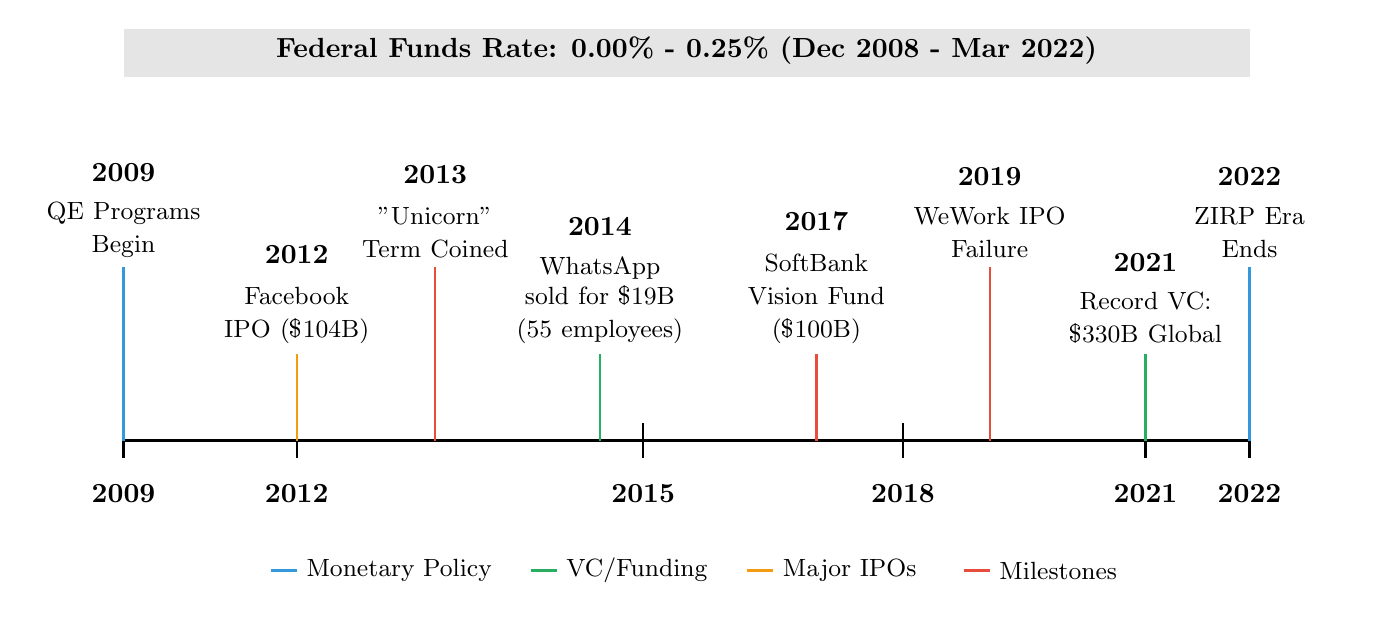
\begin{tikzpicture}[scale=1.1]
    % Define colors
    \definecolor{policyblue}{RGB}{52, 152, 219}
    \definecolor{fundinggreen}{RGB}{39, 174, 96}
    \definecolor{ipoorange}{RGB}{243, 156, 18}
    \definecolor{milestonereds}{RGB}{231, 76, 60}
    
    % Timeline base - proportional to actual years
    \draw[very thick] (0,0) -- (13,0);
    
    % Year markers - proportional spacing (1 unit = 1 year)
    \foreach \x/\year in {0/2009, 2/2012, 6/2015, 9/2018, 11.8/2021, 13/2022} {
        \draw[thick] (\x,-0.2) -- (\x,0.2);
        \node[below] at (\x,-0.4) {\textbf{\year}};
    }
    
    % Interest rate indicator at top - moved down slightly
    \fill[black!10] (0,4.2) rectangle (13,4.75);
    \node at (6.5,4.5) {\textbf{Federal Funds Rate: 0.00\% - 0.25\% (Dec 2008 - Mar 2022)}};
    
    % All events above timeline - moved down
    \node[above, text width=2.2cm, align=center] at (0,2) {
        \textbf{2009}\\[0.1cm]
        \small QE Programs\\
        \small Begin
    };
    \draw[policyblue, thick] (0,0) -- (0,2);
    
    \node[above, text width=2.2cm, align=center] at (2,1) {
        \textbf{2012}\\[0.1cm]
        \small Facebook IPO (\$104B)
    };
    \draw[ipoorange, thick] (2,0) -- (2,1);
    
    \node[above, text width=2.3cm, align=center] at (11.8,1) {
        \textbf{2021}\\[0.1cm]
        \small Record VC:\\
        \small \$330B Global
    };
    \draw[fundinggreen, thick] (11.8,0) -- (11.8,1);
    
    \node[above, text width=2.2cm, align=center] at (13,2) {
        \textbf{2022}\\[0.1cm]
        \small \ac{ZIRP} Era\\
        \small Ends
    };
    \draw[policyblue, thick] (13,0) -- (13,2);
    
    \node[above, text width=2.2cm, align=center] at (3.6,2) {
        \textbf{2013}\\[0.1cm]
        \small "Unicorn" Term Coined
    };
    \draw[milestonereds, thick] (3.6,0) -- (3.6,2);
    
    \node[above, text width=2.5cm, align=center] at (5.5,1) {
        \textbf{2014}\\[0.1cm]
        \small WhatsApp sold for \$19B\\
        \small (55 employees)
    };
    \draw[fundinggreen, thick] (5.5,0) -- (5.5,1);
    
    \node[above, text width=2.2cm, align=center] at (8,1) {
        \textbf{2017}\\[0.1cm]
        \small SoftBank Vision Fund (\$100B)
    };
    \draw[milestonereds, thick] (8,0) -- (8,1);
    
    \node[above, text width=2.2cm, align=center] at (10,2) {
        \textbf{2019}\\[0.1cm]
        \small WeWork IPO\\
        \small Failure
    };
    \draw[milestonereds, thick] (10,0) -- (10,2);
    
    % Legend - positioned below timeline with better spacing
    \begin{scope}[shift={(1.5,-1.5)}]
        \draw[policyblue, thick] (0.2,0) -- (0.5,0);
        \node[right] at (0.5,0) {\small Monetary Policy};
        
        \draw[fundinggreen, thick] (3.2,0) -- (3.5,0);
        \node[right] at (3.5,0) {\small VC/Funding};
        
        \draw[ipoorange, thick] (5.7,0) -- (6,0);
        \node[right] at (6,0) {\small Major IPOs};
        
        \draw[milestonereds, thick] (8.2,0) -- (8.5,0);
        \node[right] at (8.5,0) {\small Milestones};
    \end{scope}
    
\end{tikzpicture}
\caption{Timeline of the Zero Interest-Rate Policy Era (2009-2022)}
\label{fig:zirp_timeline}
\end{figure}

\subsection{Operationalizing Venture Success}

The staged nature of venture capital provides a natural framework for measuring startup performance. Securing a subsequent funding round is a clear, binary indicator of success, signifying that a company has met the milestones required to attract further investment. Beyond this binary outcome, the funding growth rate—the percentage increase in capital raised between rounds—serves as a continuous measure of investor confidence and perceived value creation.

These funding-based metrics are well-established proxies for startup success in the venture ecosystem \citep{gompers2001venture}. They represent the revealed preferences of sophisticated investors who have conducted due diligence and are "voting with their wallets." Unlike more subjective measures, funding outcomes are objective, quantifiable, and directly reflect the market's assessment of a startup's progress and future potential. Critically, these metrics capture the market's implicit valuation of the speed-versus-quality trade-offs that startups make—providing an external validation mechanism for strategies that prioritize development velocity over traditional engineering best practices.

\section{Synthesis, Research Gap, and Limitations}\label{sec:lit_gap}

The literature from software engineering and venture capital presents a direct and fundamental conflict regarding the strategic management of technical debt in startups. Software engineering research extensively documents the negative long-term impacts of technical debt, framing it as a liability to be rigorously managed for sustainable development \citep{colazo2010collaboration, arcelli2012investigating}. This traditional engineering perspective emphasizes that debt accumulation inevitably leads to decreased velocity, increased maintenance costs, and systemic fragility that threatens long-term viability.

The strategic calculus surrounding technical debt varies depending on financing structure. Debt-financed ventures face fixed repayment obligations that prioritize cash flow stability, while bootstrapped companies retain autonomy to optimize for sustainability \citep{levesque2000effects}. This thesis focuses on venture capital financing because it creates extreme time pressure: \ac{VC} funds operate on finite horizons requiring portfolio companies to achieve substantial scale within compressed timeframes, intensifying the velocity imperative beyond other funding mechanisms \citep{gompers2001venture}.

In sharp contrast to engineering wisdom, the prevailing narrative in entrepreneurship and \ac{VC} literature, particularly from the \ac{ZIRP} era, emphasizes that for equity-backed companies, speed, momentum, and market traction are the primary determinants of survival and access to capital \citep{kuratko2020blitzscaling}. This temporal constraint creates explicit incentives for rapid execution that directly oppose traditional engineering wisdom about sustainable development practices. The costs of being slow to market in VC-backed ventures—missed competitive windows, diminished investor interest, lost first-mover advantages—are perceived to far outweigh the future costs of technical debt accumulation. The \ac{VC} ecosystem's explicit reward structure thus creates a strategic environment fundamentally different from debt-financed or bootstrapped alternatives.

This tension reveals a critical conceptual gap: established engineering models for quality management fail to account for the unique incentive structures, competitive dynamics, and survival pressures facing equity-backed ventures operating under compressed exit timelines. The traditional debt metaphor, which assumes that "interest payments" will eventually constrain growth, may not hold when external capital can continuously subsidize the costs of poor code quality, and when market timing constraints make speed existentially important.

A significant empirical research gap exists at this intersection. There is a lack of large-scale, quantitative research examining the relationship between technical debt, development velocity, and funding outcomes for startups during periods of capital abundance. Most technical debt studies focus on mature organizations with stable revenue streams, or rely on methodologies not suited for cross-company comparison \citep{li2015systematic}. This has left the strategic debate dominated by anecdote and theoretical frameworks rather than systematic empirical evidence about how these trade-offs actually play out in practice.

This thesis directly addresses this gap by providing a large-scale, quantitative analysis of the relationship between objectively measured technical debt, development velocity, and funding success during the capital-abundant \ac{ZIRP} era. The research design faces inherent limitations, including sample selection constraints, measurement validity concerns, and temporal specificity, which are addressed in detail in the methodology (Section \ref{sec:methodology}) and discussed with respect to generalizability and future research directions in Section \ref{subsec:boundaries}.

Despite these limitations, this study provides a critical empirical foundation for moving beyond the theoretical tensions between engineering and venture perspectives toward a more nuanced, context-aware understanding of technical debt's strategic role in venture execution. The research aims to determine whether the traditional engineering view of debt as liability holds under the unique conditions of venture-backed growth, or whether debt might indeed represent a strategic tool for market capture during periods of abundant capital.